%Abtasttheorem und diskrete Fouriertransformation

\section{Abtasttheorem, diskrete Fouriertransformation}
	\begin{minipage}{12cm}
		Abtasten einer Funktion mit idealem Abtaster und Abtastintervall $\Delta t$.\\
		$ \scalebox{1.2}{$f(t) \cdot \delta_{\Delta t}(t) = \sum\limits_{k=-\infty}^{\infty} \Delta t \cdot f(k \Delta t) \cdot \delta(t-k \Delta t) $}$
	\end{minipage}
	\begin{minipage}{6cm}
		\begin{tabular}{|l l l|}
			\hline
				Periodisieren &$\laplace$ & Abtasten\\
				Abtasten & $\laplace$ & Periodisieren\\
			\hline
		\end{tabular}
	\end{minipage}

\subsection{Abtasttheoreme}
	\textbf{Kardinalreihe:}  $\scalebox{1.2}{$S(\omega) = \sum\limits_{k=-\infty}^{\infty} S(k\frac{\pi}{T}) \cdot \frac{\sin(\omega T - k\pi)}{\omega T - k\pi}$
	mit $S(k\frac{\pi}{T}) = 2Tc_k$}$\\

	\textbf{Abtasttheorem f\"ur die Frequenz:}
	F\"ur ein Signal von endlicher Dauer $2T$ ist die Fouriertransformierte durch ihre Abtastwerte an den Stellen $k\frac{\pi}{T}$
	vollst\"andig bestimmt. \\
	
	\textbf{Abtasttheorem von Shannon:}
	Ist ein Signal bandbegrenzt mit Grenzfrequenz $\omega_g$, so l\"asst sich das Signal anhand der Abtastwerte zu den Zeitpunkten
	$k\frac{\pi}{\omega_g}$ vollst\"andig rekonstruieren.
	
	
\subsection{Diskrete Fouriertransformation}
\begin{minipage}{14cm}
	mit $N$ Abtastpunkten\\
	-	Die DFT liefert nur $\frac{N}{2}$ unabh\"angige Koeffizienten, da $\hat{c_k}$ und $\hat{c_{-k}}$ konjugiert komplex sind.\\
	- Die Abtastfrequenz muss mindestens doppelt so gross sein, wie der zu beobachtende Frequenzinhalt...
\end{minipage}
\begin{minipage}{6cm}
	$$\hat{c_k} = \frac{1}{N} \cdot \sum\limits_{n=0}^{N-1} y_n \cdot e^{-jkn\frac{2\pi}{N}}$$
\end{minipage}
	
	
	
	
\subsection{Alias-Effekt}

	Ist die Abtastfrequenz zu klein, k\"onnen die Frequenzen nicht mehr sauber getrennt werden, der sogenannte Alias-Effekt tritt auf:
	die Anteile aller Frequenzen werden der jeweils betragsm\"assig kleinsten passenden Frequenz zugeordnet.
	
	\begin{minipage}[c]{8.5cm}
		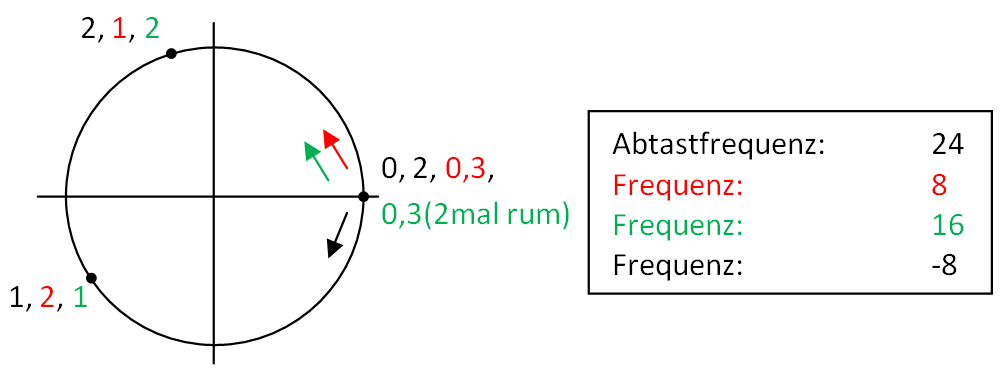
\includegraphics[width=8cm]{./bilder/Alias-effekt.png}
	\end{minipage}
	\begin{minipage}[c]{8cm}
		Summeneigenschaft: $\hat{c_k} = \sum\limits_{m=-\infty}^{\infty} c_{k+mN}$
	\end{minipage}
	%\begin{tabular}{p{8.5cm} p{5cm}}
	%	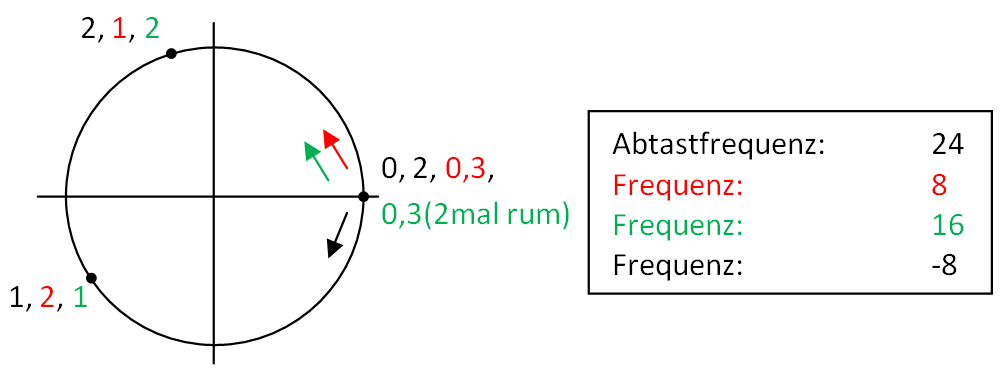
\includegraphics[width=8cm]{./bilder/Alias-effekt.png} & Summeneigenschaft: $\hat{c_k} = \sum\limits_{m=-\infty}^{\infty} c_{k+mN}$
	%\end{tabular}
	
